\section{Einführung}
Soll ein Gas der Stoffmenge $\nu$ bei konstantem Volumen um $dT$ erwärmt werden, so muss die Wärme 
\begin{equation}
	\delta Q_V=\nu\, c_{m,V}\, dT
\label{eq:cv}
\end{equation}
zugeführt werden. Dabei ist $c_{m,V}$ die molare Wärmekapazität bei konstatem Volumen.
Wird stattdessen der Druck konstant gehalten, bekommt man mit der molaren Wärmekapazität bei konstantem Druck $c_{m,p}$ die Gleichung
\begin{equation}
	\delta Q_p=\nu\, c_{m,p}\, dT\qquad .
\label{eq:cp}
\end{equation}

Es gilt mit der universellen Gaskonstant $R$:
\begin{equation}
	c_{m,p} - c_{m,V}=R
\label{eq:cvminuscp}
\end{equation}

Die Anzahl der Freiheitsgerade $f$ eines Moleküls ist die Anzahl der unabhängigen Koordinaten, mit denen der Bewegungszustand des Moleküls vollständig beschrieben wird. Aus 
\begin{equation}
	c_{m,V}=\frac{f}{2}R\qquad c_{m,p}=\frac{f+2}{f}R
\label{eq:freiheit}
\end{equation}
berechnet sich der Adiabatenexponent $\kappa$ zu 
\begin{equation}
	\kappa=\frac{c_{m,p}}{c_{m,V}}=\frac{f+2}{f}
\label{eq:kappa}
\end{equation}

Eine \textbf{adiabatische Zustandsänderung} eines Gases liegt vor, wenn kein Wärmeaustausch mit der Umgebung stattfindet. Dies ist näherungsweise erfüllt bei guter Wärmeisolierung des Systems gegen die Umgebung bzw. schneller Prozessführung. Es lassen sich die Poissonschen Gleichungen herleiten:

\begin{align}
	T\cdot V^{\kappa-1}&=\text{const}' \\
	p\cdot V^{\kappa}&=\text{const}'' \\
	\frac{T^{\kappa}}{p^{\kappa-1}}&=\text{const}'''
\label{eq:poisson}
\end{align}
Es wurde mit zwei Versuchen der Adiapatenexponent $\kappa$ bestimmt:
\subsection{Bestimmung nach Rüchardt-Flammersfeld}
\begin{figure}[h]
  \centering
  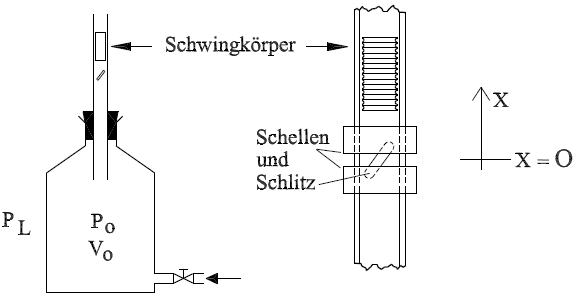
\includegraphics[width=.7\textwidth]{res/ruechardt}
  \caption{"Versuchsaufbau zur $\kappa$-Bestimmung nach Rüchardt-Flammersfeld"\footcite{anleitung-ss2015}}
  \label{fig:ruechardt}
\end{figure}
Das Gas ist in einer Flasche mit aufgesetztem Glasrohr gefüllt. Dieses Glasrohr hat auf der Hälfte der Länge einen Schlitz einstellbarer Größe.
Ein Schwingkörper der Masse $m$ und Durchschnittsfläche $A$ schwingt auf der Höhe des Schlitzes, während unten Gas nachströmt (Kompensation von Reibungsverlusten bei der Schwingung).
In Ruheposition des Schwingkörpers setzt sich der Innendruck $p_0$ aus dem Außendruck $p_L$ und dem Druck durch Gewichtskraft des Schwingkörpers zusammen (Erdbeschleunigung $g$):
\begin{equation}
	p_0=p_L+\frac{m\cdot g}{A}
\label{eq:p0}
\end{equation}
Die Schwingung entsteht aufgrund von oszillatorischer Komprimierung / Dekomprimierung des Gases durch die Bewegung des Schwingkörpers und dieser folgt der Bewegungsgleichung
\begin{equation}
	m\,\frac{\di^2 x}{\di t^2}=-\frac{\kappa p_0 A^2}{V_0}x\qquad ,
\label{eq:bwgl}
\end{equation}
wobei $V_0$ das Volumen des Gases in Ruheposition des Schwingkörpers ist. $\kappa$ wird aus der Periodendauer $T$ der Schwingung bestimmt:
\begin{equation}
	\kappa=\frac{4\pi^2 m V_0}{p_0 A^2 T^2}
\label{eq:ruechardt}
\end{equation}
\subsection{Bestimmung nach Clément-Desormes}
\begin{figure}[h]
  \centering
  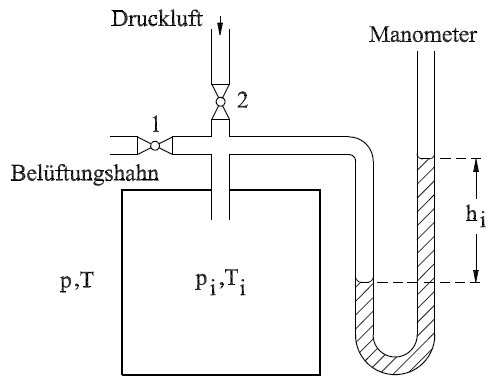
\includegraphics[width=.7\textwidth]{res/clement}
  \caption{"Versuchsaufbau zur $\kappa$-Bestimmung nach Clément-Desormes"\footcite{anleitung-ss2015}}
  \label{fig:clement}
\end{figure}
Die Luft ist in einen gut isolierten Behälter gefüllt. Der Innendruck wird über die Höhe $h$ einer Flüssigkeit im Manometer abgelesen. Über ein erstes Rohr kann durch Öffnen eines Hahns (1) Druckausgleich mit der Außenluft hergestellt werden, über ein zweites kann Druckluft mit einer Handpumpe zugeführt werden (Hahn 2).

Zuerst wird über Rohr 2 Luft zugepumpt, sodass der Innendruck höher als der Außendruck ist. Hierbei erwärmt sich die Luft. Hahn 2 wird geschlossen und gewartet, bis wieder Temperaturgleichgewicht zur Außenluft herrscht. Nun wird die Höhe $h_1$ am Manometer abgelesen.

Hahn 1 wird nun gerade schnell genug geöffnet und wieder geschlossen, dass der Druck sich ausgleicht. Die Luft durchläuft eine annähernd adiabatische Zustandsänderung und kühlt sich ab. Nach Schließen des ersten Hahnes wartet man auf Temperaturausgleich, wobei der Druck steigt (das Volumen bleibt hierbei konstant, da beide Hähne geschlossen sind). Ist dies geschehen, liest man $h_3$ am Manometer ab.

Der Adiabatenkoeffizient errechnet sich dann aus
\begin{equation}
	\kappa=\frac{h_1}{h_1-h_3} \qquad .
\label{eq:clement}
\end{equation}

\section{Versuch}
\subsection{Bestimmung nach Rüchardt-Flammersfeld}
Der Versuch wurde wie in der Einführung beschrieben mit Luft, Argon und $\mathrm{CO}_2$ durchgeführt. Dazu wurden pro Gas für 5 verschiedene Schlitzbreiten je 100 Schwingungen gemessen. An den Werten in \cref{tab:ruechluft} kann kein von der Spaltenbreite abhängiger Trend erkannt werden, darum ist ein Fit nicht sinnvoll. Wir rechnen stattdessen mit dem Mittelwert aller 5 Messungen: $\kappa_L=\num{1.39(10)}$, was einem Freiheitsgrad von $f_L=2/(\kappa-1)=\num{5.13(131)}$ entspricht.
\begin{table}[H]
\centering
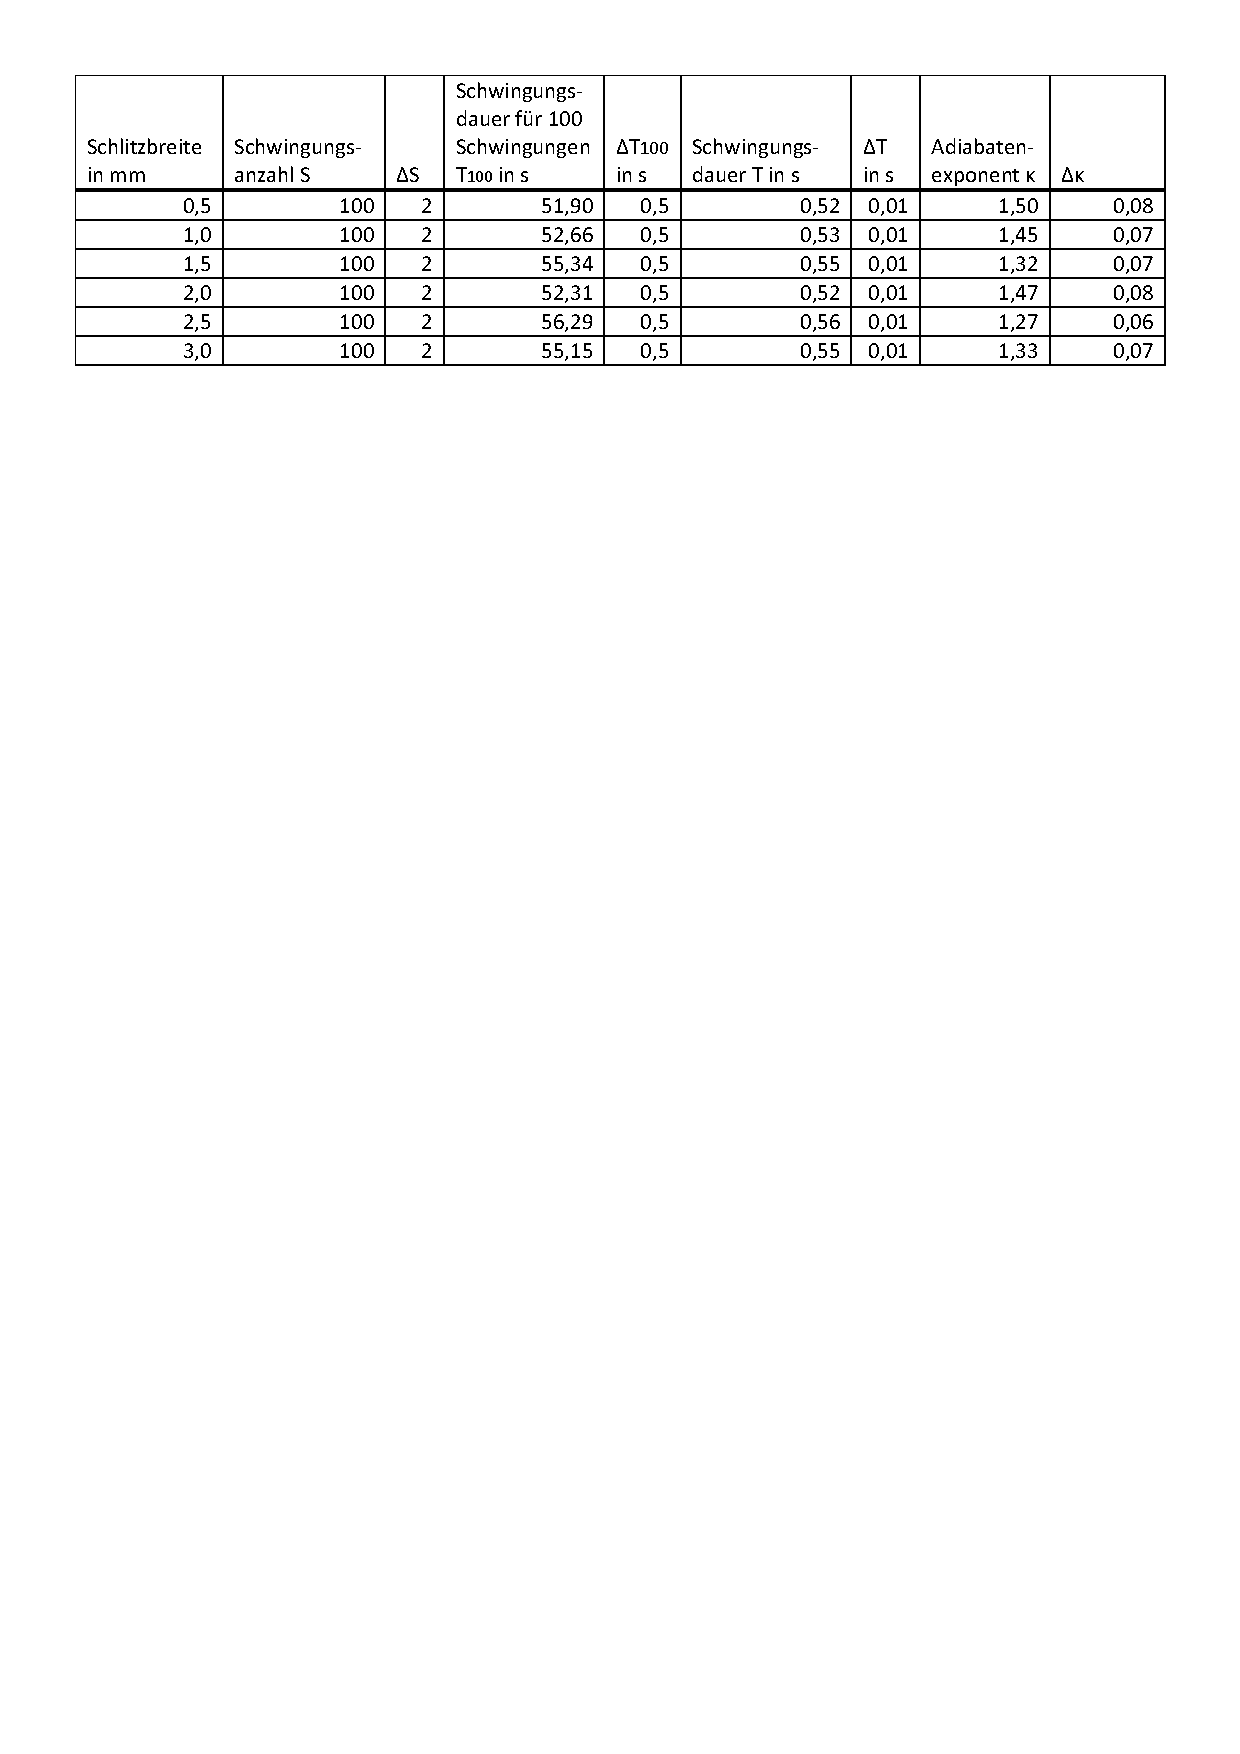
\includegraphics[width=0.6\linewidth,trim=5cm 23cm 5cm 1cm]{res/Luft}
\caption{Bestimmung von $\kappa$ für Luft nach dem Rüchardt-Flammersfeld-Verfahren.}
\label{tab:ruechluft}
\end{table}

Bei Argon und $\mathrm{CO}_2$ scheinen die Werte für verschiedene Schichtbreiten innerhalb des Fehlers konstant zu bleiben. Auch hier nehmen wir deshalb den Mittelwert: $\kappa_{Ar}=\num{1.66(9)}$, $\kappa_{\mathrm{CO}_2}=\num{1.31(7)}$. Daraus ergeben sich die Freiheitsgerade $f_{Ar}=\num{3.03(41)}$ bzw. $f_{\mathrm{CO}_2}=\num{6.45(146)}$.
\begin{table}[h]
\centering
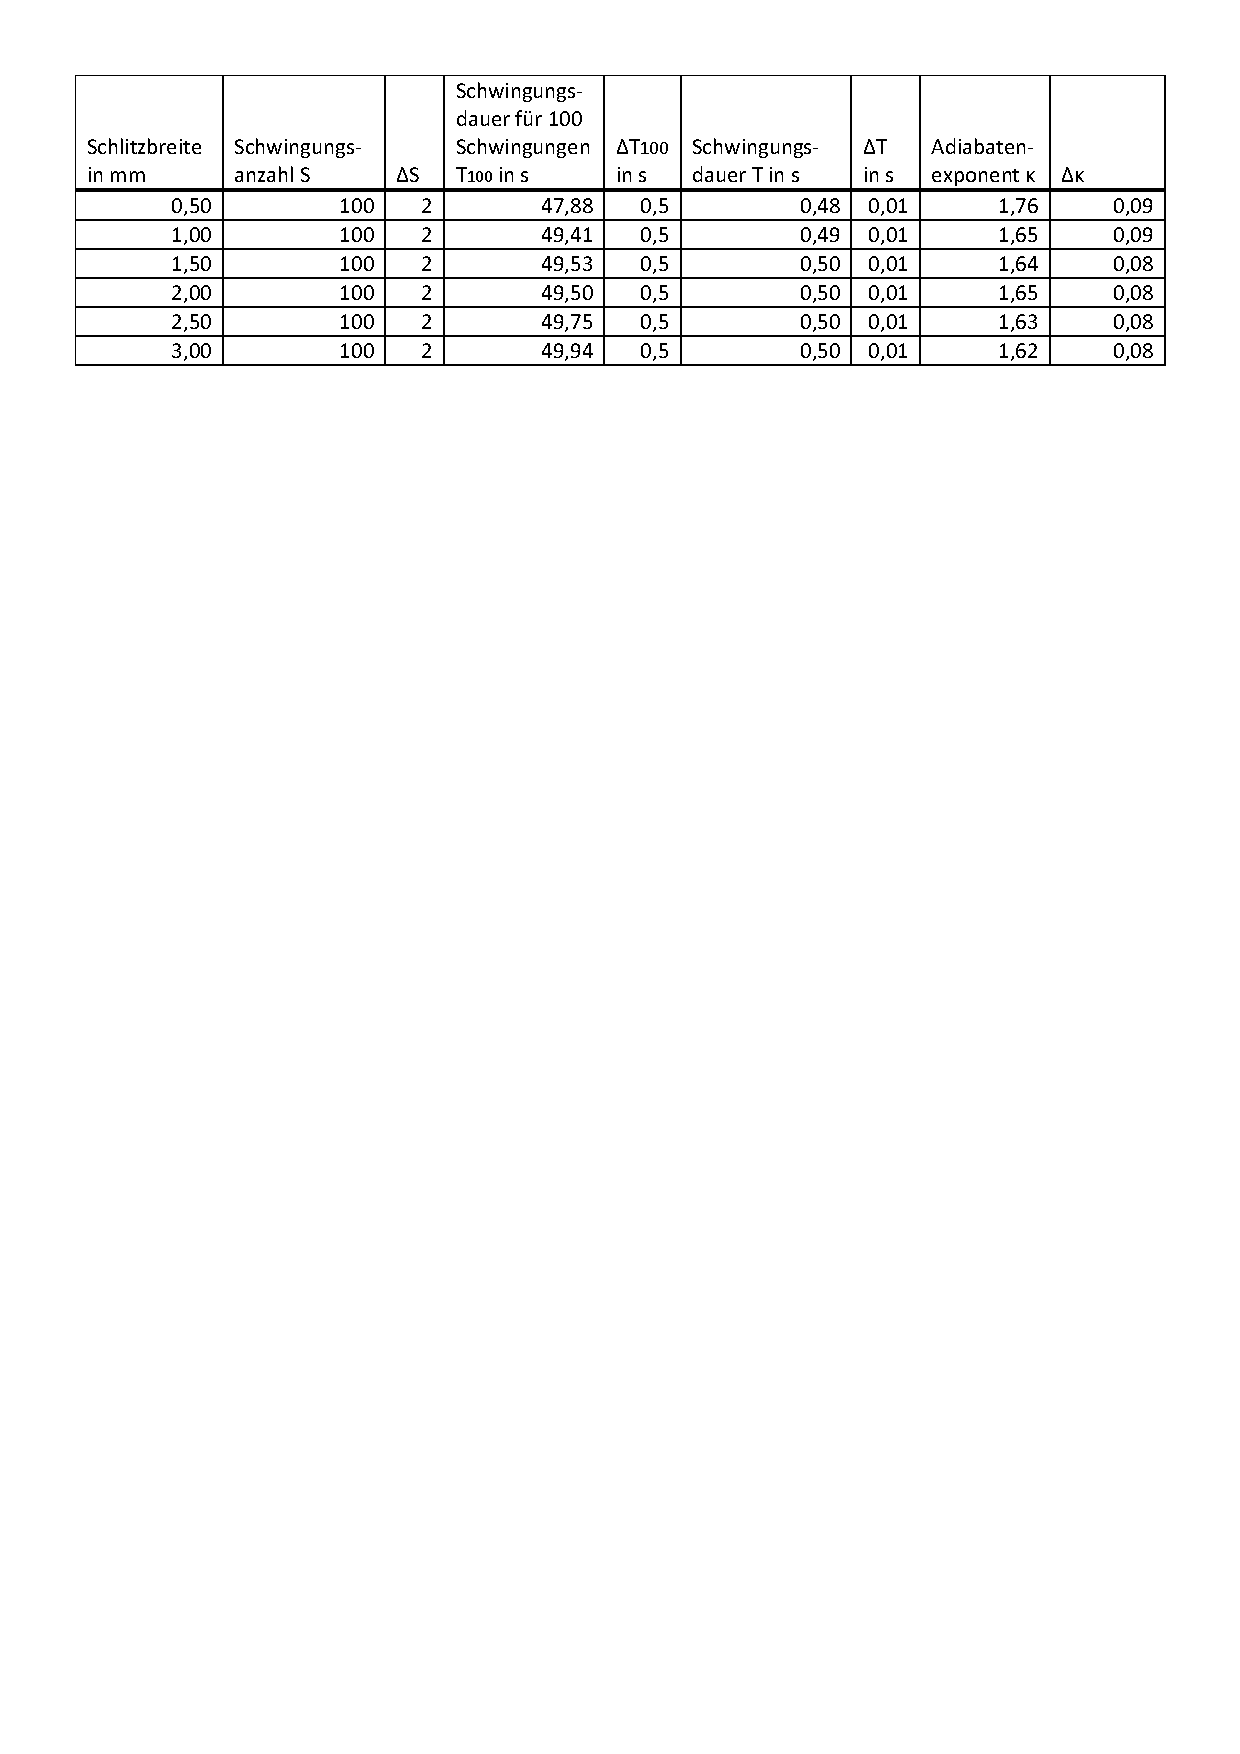
\includegraphics[width=0.6\linewidth,trim=5cm 23cm 5cm 1cm]{res/Argon}
\caption{Bestimmung von $\kappa$ für Argon nach dem Rüchardt-Flammersfeld-Verfahren.}
\label{tab:ruechargon}
\end{table}

\begin{table}[h]
\centering
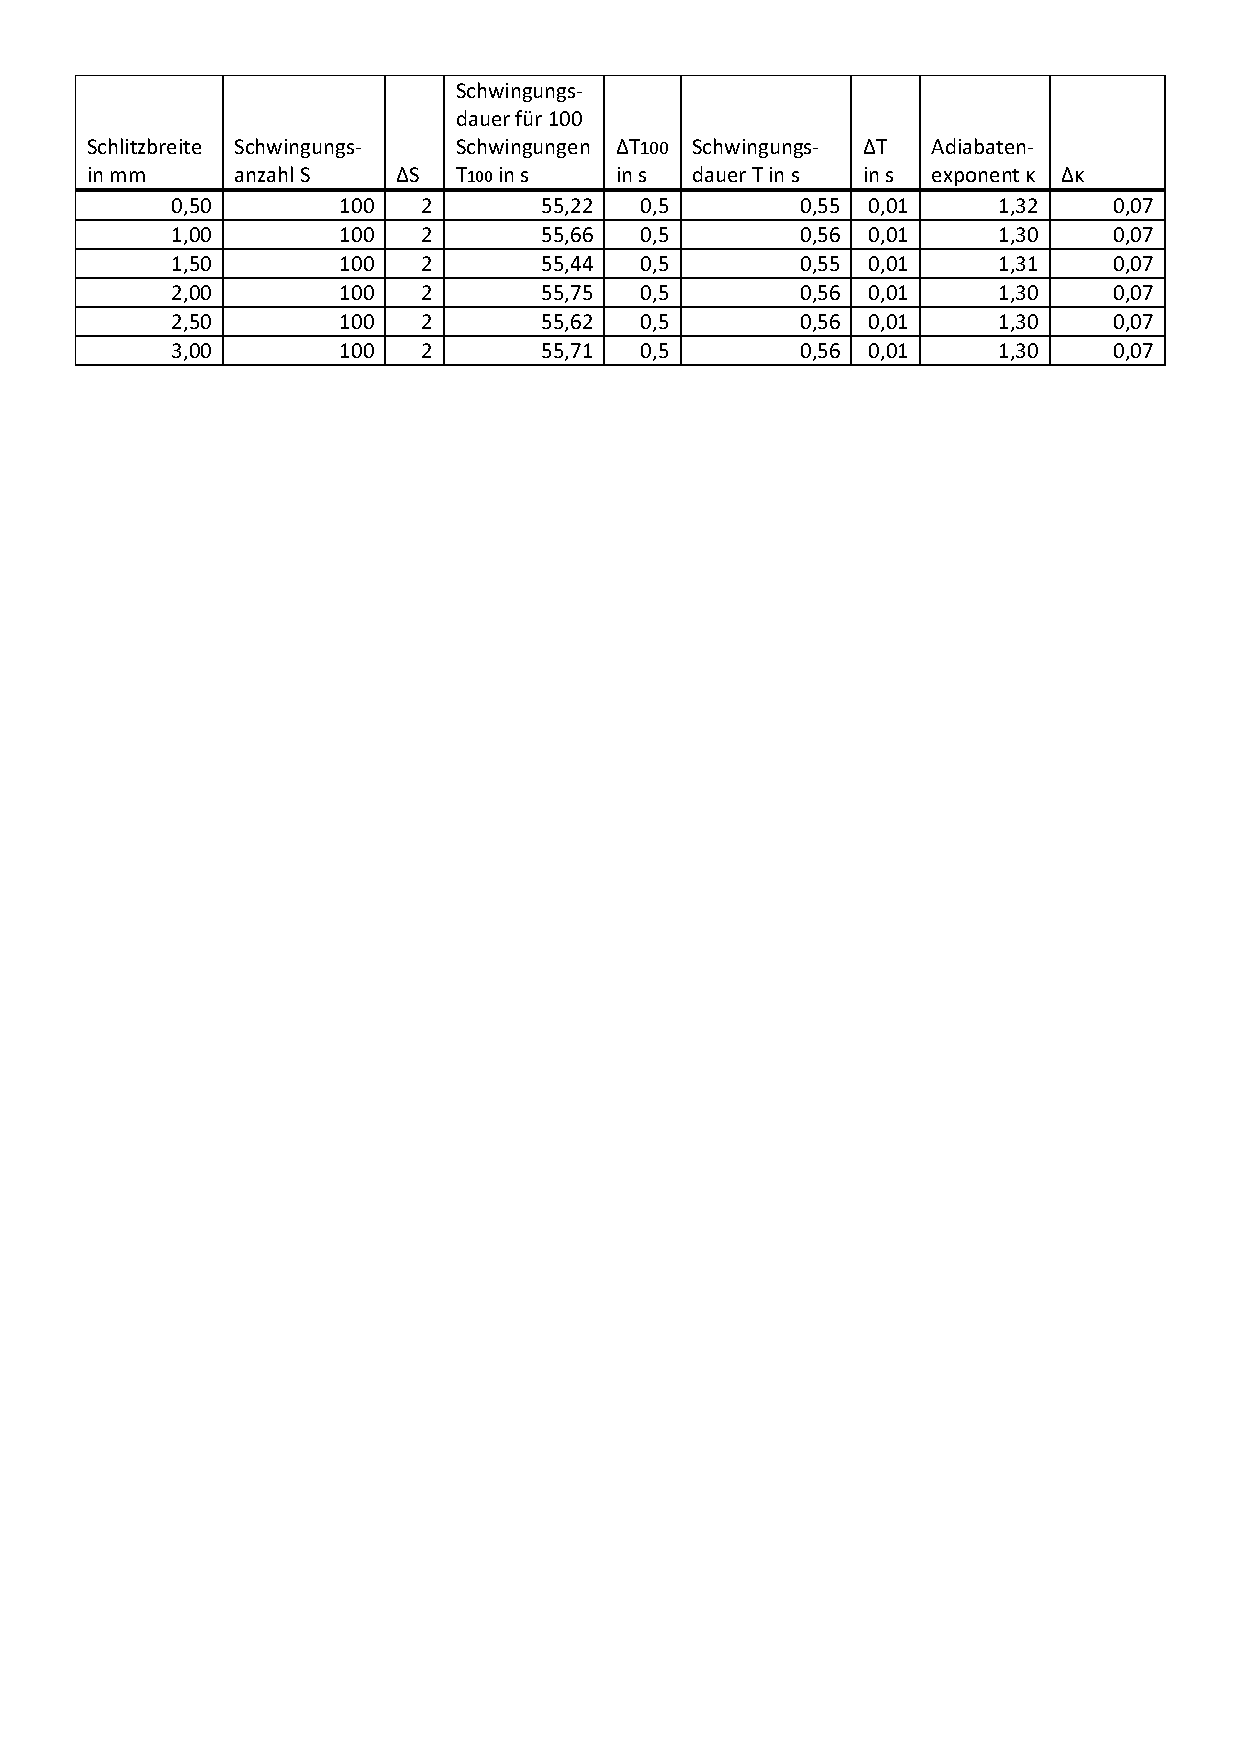
\includegraphics[width=0.6\linewidth,trim=5cm 23cm 5cm 1cm]{res/CO2}
\caption{Bestimmung von $\kappa$ für $\mathrm{CO}_2$ nach dem Rüchardt-Flammersfeld-Verfahren.}
\label{tab:ruechco2}
\end{table}

\subsection{Bestimmung nach Clément-Desormes}
Der Versuch wurde 6 mal durchgeführt. Allerdings wurde ein Ablesefehler begangen: es wurde nicht die Höhendifferenz zwischen den beiden Flüssigkeitssäulen am Manometer abgelesen, sondern nur der Skalenwert der rechten Säule. Da der Skalenwert bei ausgeglichenem Druck nicht bekannt ist, lässt sich $\kappa$ hieraus nicht bestimmen (die Werte in \cref{tab:clementluft} sind offensichtlich deutlich zu hoch).

Wir nehmen stattdessen einen Literaturwert für $\kappa$ und rechnen rückwärts, was der Skalenwert $H_0$ am Manometer bei ausgeglichenem Druck wäre. Sind $\Delta h_1$ und $\Delta h_3$ die eigentlich benötigten Skalendifferenzen zwischen den Säulen und $h_1$ bzw. $h_3$ die von uns abgelesenen Skalenwerte der rechten Säule, so gilt
\begin{align}
	\Delta h_1&=2(h_1-H_0)\qquad \Delta h_3=2(h_3-H_0) \\
	\kappa&=\frac{\Delta h_1}{\Delta h_1-\Delta h_3}=\frac{h_1-H_0}{h_1-h_3}\\
	\implies H_0&=(h_3-h_1)\kappa+h_1\qquad .
\label{eq:hoehe}
\end{align}
Mit $\kappa=\num{1.40}$\footcite[][827]{white} bekommen wir $H_0=\SI{38.8(3)}{cm}$.
\begin{table}[h]
\centering
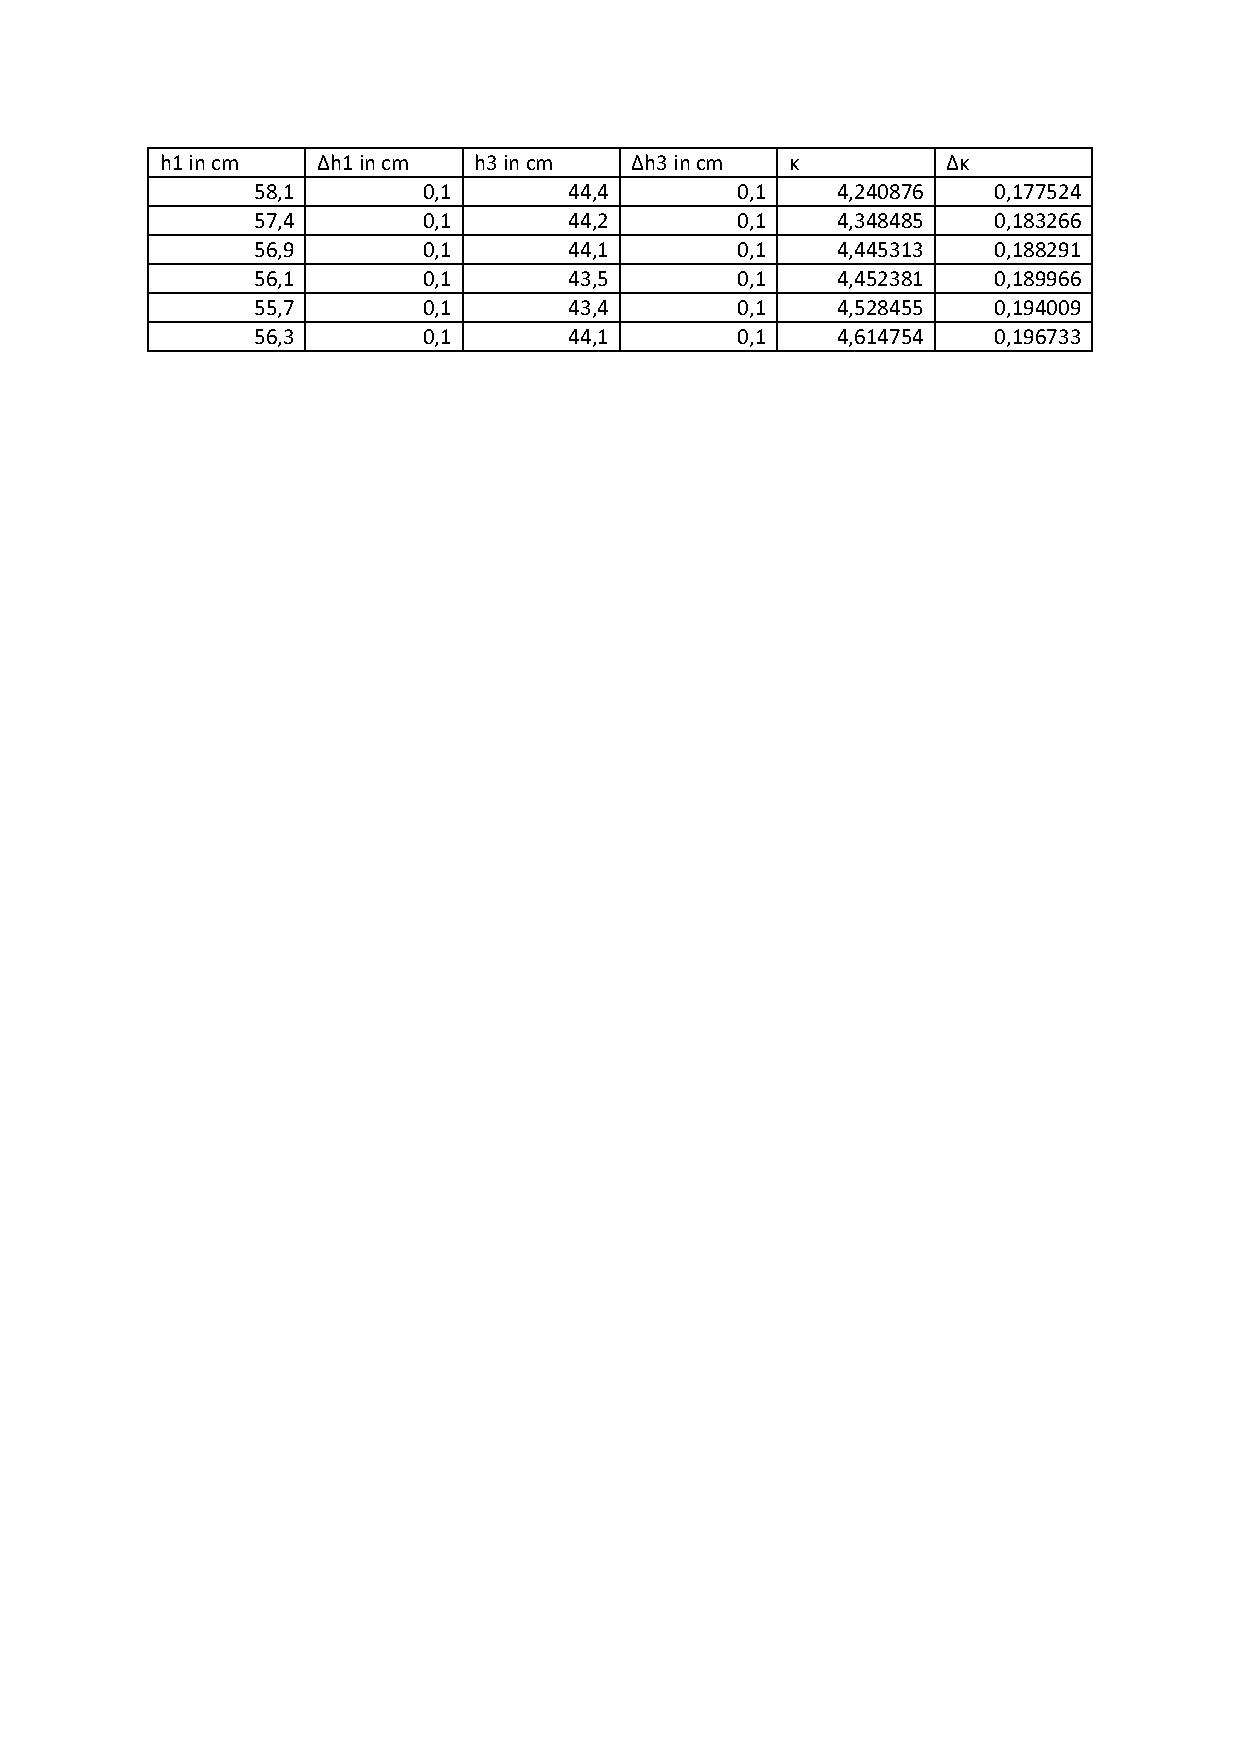
\includegraphics[width=0.6\linewidth,trim=5cm 23cm 5cm 1cm]{res/Luft2}
\caption{Bestimmung von $\kappa$ für Luft nach dem Clément-Desormes-Verfahren.}
\label{tab:clementluft}
\end{table}

\section{Diskussion}
Im Verfahren nach Rüchardt-Flammersfeld wurden folgende Werte bestimmt:
\begin{table}[H]
\centering
\begin{tabular}{c | c c c}
		Gas & $\kappa$ gemessen & $\kappa$ Literaturwert & $f$ gemessen  \\ \midrule
		Luft & \num{1.39(10)} & \num{1.40} & \num{5.13(131)} \\
		Argon & \num{1.66(9)} & \num{1.67} & \num{3.03(41)} \\
		$\mathrm{CO_2}$ & \num{1.31(7)} & \num{1.30} & \num{6.45(146)}
\end{tabular}
\caption{Gegenüberstellung der gemessenen Werte zu Literaturwerten nach \citeauthor{white}}
\label{tab:litwerte}
\end{table}
Die Übereinstimmung mit den Literaturwerten ist sehr gut. In \cref{fig:freiheit} sind Freiheitsgrade für verschiedene Gasatome aufgelistet. 

Argon ist ein einatomiges Gas und hat 3 Freiheitsgerade (Translation in 3 Raumrichtungen), was auch unserem Messwert entspricht. Luft besteht zu \SI{78}{\percent} aus Stickstoff, welches als zweiatomiges Gas 5 relevante Freiheitsgrade hat. Innerhalb des Fehlers deckt sich auch dies mit dem Messwert. 

$\mathrm{CO_2}$ ist ein gestrecktes dreiatomiges Gas, sollte also laut \cref{fig:freiheit} 5 Freiheitsgerade haben. Dies liegt gerade noch im (großen) Fehlerbereich unseres Messwertes, allerdings könnten auch einige der eingeklammerten Schwingungsmoden angeregt worden sein.

\begin{figure}[h]
  \centering
  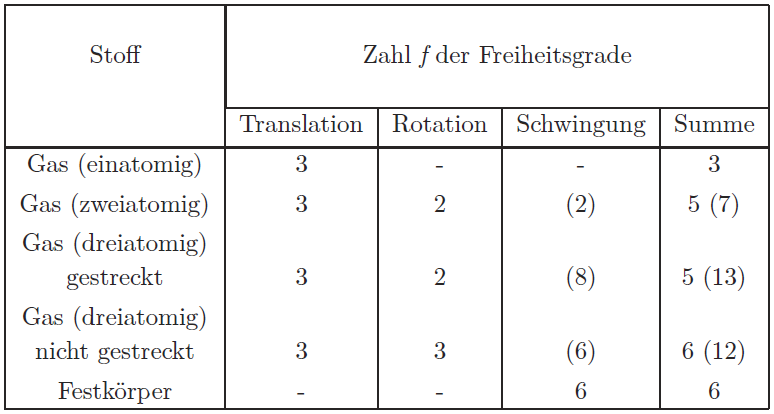
\includegraphics[width=.75\textwidth]{res/freiheit}
  \caption{"Zahl $f$ der anregbaren Freiheitsgrade. Die eingeklammerten Schwingungsfreiheitsgrade sind bei Raumtemperatur meist nicht angeregt."\footcite{anleitung-ss2015}}
  \label{fig:freiheit}
\end{figure}